%!TEX root = ../Tesis_Luis_Gomez.tex
\chapter{Introducción específica}

\section{Componentes Principales del Hardware}

\subsection{Destalles del equipo, la tecnología del sensor y muestreo estadístico}

En la figura \ref{fig:diagBloques}, se presenta el diagrama en bloques del instrumento. En él, se puede apreciar un microcontrolador central responsable de gestionar: tres sensores de MP2,5, encargados de medir el contaminante; un sistema de almacenamiento de datos local y un sistema encargado de la transmisión de los registros hacia un servidor remoto. Además, incluye un reloj de tiempo real (RTC) que registra el momento de cada medición y un sistema de alimentación, compatible con la red eléctrica.

\begin{figure}[htpb]
    
	\centering
	\shorthandoff{<>} % Desactivar caracteres problemáticos
	\begin{tikzpicture}[ node distance=1cm]
	% Nodes
	\node (microcontroller)
	[draw, rectangle, fill=blue!10!white, align=center]
	{\textbf{Microcontrolador}\\ \rotatebox{90}{\faMicrochip}};

	\node (sensor1)
	[above right=of microcontroller, draw, rectangle, fill=red!10!white, align=center, yshift=0.2cm, xshift=0.3cm]
	{Sensor de\\MP2,5 \faSmog};

	\node (sensor2)
	[right=of microcontroller, draw, rectangle, fill=red!10!white, align=center]
	{Sensor de\\MP2,5 \faSmog};

	\node (sensor3)
	[below right=of microcontroller, draw, rectangle, fill=red!10!white, align=center, , yshift=-0.2cm, xshift=0.3cm]
	{Sensor de\\MP2,5 \faSmog};

	\node (storage)
	[below=of microcontroller, draw, fill=yellow!10!white, rectangle, align=center]
	{Sistema de \\ almacenamiento  \faSdCard }; % \faDatabase

	\node (transmission)
	[above=of microcontroller, draw, rectangle, align=center]
	{Sistema de transmi-\\sión de datos  \faSignal};

	\node (rtc)
	[above left=of microcontroller, draw, rectangle, align=center, yshift=-1.5cm, xshift=-.33cm]
	{RTC \faClock[regular]};

	\node (power)
	[below left=of microcontroller, draw, rectangle, align=center,yshift=-0.2cm, xshift=0.0cm]
	{Fuente de\\poder \faBatteryQuarter};

	\node (cabinet) 		[above right=of transmission,  xshift=-6.8cm,yshift=-0.7cm]     {\textbf{Gabinete} \faCloudSunRain};

	% Bounding Box
	\begin{scope}[on background layer]
	\node[fill=gray!10,  draw, rectangle, rounded corners, fit=(cabinet) (sensor2) (rtc) (storage) (transmission)] {};
	\end{scope}

	% Arrows
	\draw[<->] (microcontroller) -- (sensor1);
	\draw[<->] (microcontroller) -- (sensor2);
	\draw[<->] (microcontroller) -- (sensor3);
	\draw[<->] (microcontroller) -- (storage);
	\draw[<->] (microcontroller) -- (transmission);
	\draw[->] (rtc) -- (microcontroller);
	\draw[->] (power) -- (microcontroller);
	\end{tikzpicture}
	\shorthandon{<>} % Reactivar caracteres problemáticos
	\caption{Esquema de bloques del instrumento.}

	\label{fig:diagBloques}
\end{figure}


\subsection{Plataforma de Desarrollo y Microcontrolador}

Se incluye en el proyecto una placa STM32 NUCLEO-F429ZI (\ref{fig:placanucleof429zi}), perteneciente a la serie Nucleo-144, diseñada para facilitar el prototipado rápido con microcontroladores STM32. Equipada con el microcontrolador STM32F429ZI, la placa ofrece características avanzadas como una unidad de punto flotante (FPU), amplia memoria y diversos periféricos integrados. La compatibilidad con la interfaz ST Morpho y el sistema Arduino permite una expansión sencilla y acceso completo a señales de microcontrolador y periféricos.

Destaca la capacidad de programación y depuración a través del ST-LINK/V2-1 integrado, lo que proporciona una solución eficiente para el desarrollo de aplicaciones. Con LEDs indicadores, botones de usuario y reset, y soporte para diversas fuentes de alimentación, incluida la USB, esta placa se orienta a aplicaciones de alta demanda de procesamiento y flexibilidad en la conexión de periféricos. Es adecuada para una variedad de aplicaciones, desde prototipos de IoT hasta sistemas embebidos complejos, destacándose por su escalabilidad y robustez como plataforma de desarrollo.

La STM32 NUCLEO-F429ZI incluye numerosos puertos especializados que facilitan la conexión a dispositivos, como sensores de material particulado, esenciales en proyectos de monitoreo de calidad del aire y otras aplicaciones ambientales. Está equipada con interfaces como I2C, SPI, UART/USART, CAN y GPIOs, permitiendo la integración de múltiples sensores y dispositivos periféricos para expandir las funcionalidades del sistema conforme sea necesario.

Estas interfaces refuerzan la capacidad de escalar la solución, permitiendo la integración de una variedad de sensores y módulos. Los sensores de material particulado, que generalmente utilizan interfaces I2C o UART, pueden ser fácilmente incorporados, posibilitando la recolección de datos ambientales en tiempo real y su integración en sistemas más amplios para análisis y monitoreo.

De acuerdo al manual si el consumo de corriente total de la placa STM32 Nucleo-144 y sus shields excede los 300 mA, es obligatorio utilizar una fuente de alimentación externa, distinta al USB, para alimentar la placa. Las opciones de conexión para esta fuente de alimentación externa incluyen E5V, VIN, o +3.3 V.

Se pueden usar tres opciones diferentes para la alimentación externa:

\begin{itemize}
	\item \textbf{VIN (7 V-12 V):} Un rango de voltaje que permite alimentar la placa a través de una fuente de alimentación externa regulada. Es útil para aplicaciones que requieren más potencia de la que el USB puede suministrar.

	\item \textbf{E5V (5 V):} Otra opción de alimentación que puede ser más conveniente dependiendo de la disponibilidad de fuentes de alimentación de 5 V.

	\item \textbf{+3.3 V:} Esta opción alimenta directamente el microcontrolador STM32 y otros componentes de la placa que operan a 3.3 V. Es importante notar que, cuando se usa esta opción de alimentación, la parte ST-LINK no recibe alimentación y por lo tanto no puede ser utilizada para programación o depuración.
\end{itemize}

% TODO: \usepackage{graphicx} required
\begin{figure}
	\centering
	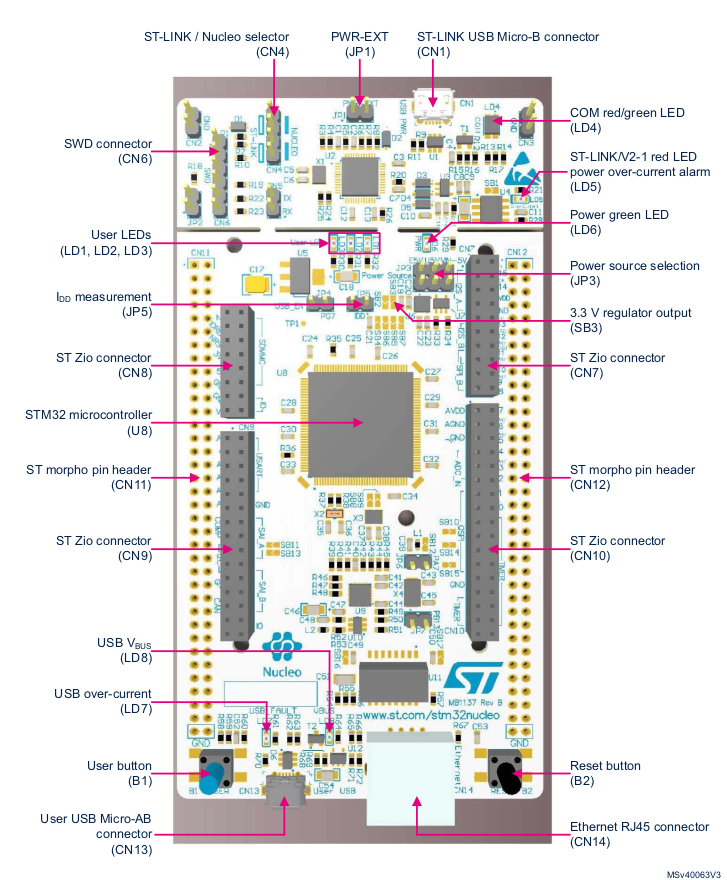
\includegraphics[width=0.7\linewidth]{Cap_02/fig/placanucleoF429ZI}
	\caption{Placa de desarrollo utilizada para el proyecto , con sus principales puertos}
	\label{fig:placanucleof429zi}
\end{figure}

\begin{table}[h]
\centering
\caption{Fuentes de alimentación externas}
\label{tab:external_power_sources}
\begin{tabular}{@{}llll@{}}
\toprule
Nombre de la entrada & Pines del conector & Rango de voltaje & Límite de corriente máxima \\ \midrule
VIN                  & CN8 pin 15, CN11 pin 24 & 7 V a 12 V       & \begin{tabular}[c]{@{}l@{}}800 mA (VIN = 7 V)\\ 450 mA (7 V < VIN < 9 V)\\ 250 mA (9 V < VIN < 12 V)\end{tabular} \\ \midrule
E5V                  & CN11 pin 6              & 4.75 V a 5.25 V  & 500 mA                    \\ \midrule
+3.3 V               & CN8 pin 7, CN11 pin 16  & 3 V a 3.6 V      & -                         \\ \bottomrule
\end{tabular}
\end{table}



\subsection{Sensores Empleados}
En esta subsección se describen los sensores utilizados en el proyecto, detallando sus características principales y el papel que desempeñan dentro del sistema.

\subsubsection{Sensor de Partículas MP25}


El SPS30, diseñado para operar  en ambientes con niveles elevados de contaminación, como áreas urbanas congestionadas o zonas industriales. Esta tecnología, facilita mediciones rápidas desde el inicio de su uso. Su vida útil, que supera los diez años. El sensor destaca por su precisión en la medición de PM2.5 y PM10, con una exactitud de ±2 µg/m³ y ±5 µg/m³ respectivamente, y por su capacidad para medir concentraciones de partículas que van desde 0.5 µg/m³ hasta 1000 µg/m³. Estas características lo hacen versátil para una amplia gama de aplicaciones, desde la monitorización de calidad del aire interior hasta la identificación de fugas en sistemas de filtración industrial.

Además, su bajo consumo energético (ver tabla) lo hace adecuado para dispositivos portátiles o aquellos alimentados por batería. La facilidad de uso y la integración en sistemas de monitoreo. Posee compatibilidad con interfaces de comunicación estándar como I2C y UART. Estas interfaces permiten la recopilación y análisis de datos ambientales, facilitando la comunicación del sensor con necesidades específicas del proyecto.

\begin{table}[H]
\centering
\caption{Características del sensor de material particulado}
\label{tab:sensor_caracteristicas}
\begin{tabular}{|l|l|}
\hline
\textbf{Característica}                              & \textbf{Valor}                         \\ \hline
Rango de medición de PM2.5                           & 0.5 µg/m³ a 1000 µg/m³                 \\ \hline
Rango de medición de PM10                            & 0.5 µg/m³ a 1000 µg/m³                 \\ \hline
Precisión de PM2.5                                   & ±5 µg/m³                               \\ \hline
Precisión de PM10                                    & ±5 µg/m³                               \\ \hline
Tiempo de respuesta                                  & 1 s                                    \\ \hline
Flujo de aire                                        & 2 L/min                                \\ \hline
Consumo máximo de energía                            & 80 mA                                  \\ \hline
Tensión de alimentación                              & 4.5 V a 5.5 V                          \\ \hline
Interfaz de comunicación                             & I2C, UART                              \\ \hline
Rango de temperatura de funcionamiento               & -20 °C a +70 °C                        \\ \hline
Rango de humedad de funcionamiento                   & 0 \% a 80 \% RH                        \\ \hline
Dimensiones                                          & 41 mm x 41 mm x 12 mm                  \\ \hline
Peso                                                 & 26 g                                   \\ \hline
\end{tabular}
\end{table}



\begin{table}[H]
\centering
\caption{Características eléctricas}
\label{tab:electrical_characteristics}
\begin{tabular}{|l|l|l|l|l|}
\hline
\textbf{Parámetro}                  & \textbf{Condiciones}                  & \textbf{Min}   & \textbf{Typ}   & \textbf{Max}   \\ \hline
Voltaje de alimentación (V)         &                                       & 4.5            & 5.0            & 5.5            \\ \hline
Corriente de suministro (µA)        & Modo sueño                            & -              & 38             & 50             \\ \hline
Corriente de suministro (mA)        & Modo inactivo                         & 300            & 330            & 360            \\ \hline
Corriente de suministro (mA)        & Modo medición                         & 45             & 55             & 65             \\ \hline
Corriente de suministro (mA)        & Primeros 200ms (iniventilador) & -              & -              & 80             \\ \hline
Voltaje de entrada nivel alto (V)   &                                       & -              & 2.31           & 5.5            \\ \hline
Voltaje de entrada nivel bajo (V)   &                                       & 0              & 2.9            & 0.99           \\ \hline
Voltaje de salida nivel alto (V)    &                                       & -              & 3.3            & 3.37           \\ \hline
Voltaje de salida nivel bajo (V)    &                                       & 0              & 0              & 0.4            \\ \hline
\end{tabular}
\end{table}


\subsubsection{Sensor de Humedad y Temperatura DHT22}

El DHT22 es un sensor digital de bajo costo que mide la temperatura y la humedad relativa del ambiente. Es un sensor popular entre los aficionados a la electrónica y los makers debido a su facilidad de uso y su bajo precio.


\begin{table}[H]
\centering
\caption{Tabla de características del sensor DHT22}
\label{tab:dht22_caracteristicas}
\begin{tabular}{|l|l|}
\hline
\textbf{Característica}                              & \textbf{Valor}                       \\ \hline
Rango de medición de temperatura                     & -40 °C a 80 °C                       \\ \hline
Precisión de temperatura                             & ±0.5 °C                              \\ \hline
Rango de medición de humedad                         & 0 \% a 100 \% HR                     \\ \hline
Precisión de humedad                                 & ±2 \% HR                             \\ \hline
Tiempo de respuesta                                  & 2 s                                  \\ \hline
Tensión de alimentación                              & 3.3 V a 5.5 V                        \\ \hline
Interfaz de comunicación                             & 1-Wire                               \\ \hline
Dimensiones                                          & 26 mm x 29 mm x 15 mm                \\ \hline
Peso                                                 & 4 g                                  \\ \hline
\end{tabular}
\end{table}


\subsubsection{Reloj de Tiempo Real (RTC) DS1307}
El DS1307 es un módulo de reloj de tiempo real que proporciona información precisa sobre la hora y la fecha. Se utiliza para marcar temporalmente los datos recopilados por los sensores, lo cual es crucial para el análisis histórico. Estos sensores, junto con el módulo RTC, forman la base del sistema de monitoreo, permitiendo la recolección y análisis detallado de datos ambientales.

\begin{table}[H]
\centering
\caption{Características del Reloj de Tiempo Real (RTC) DS1307}
\label{tab:rtc_ds1307_caracteristicas}
\begin{tabular}{|l|l|}
\hline
\textbf{Característica}                              & \textbf{Valor}                       \\ \hline
Rango de voltaje de alimentación                     & 2.0V a 5.5V                          \\ \hline
Corriente de alimentación (en funcionamiento)        & 250µA (típico)                       \\ \hline
Corriente de alimentación (en modo de espera)        & 1µA (típico)                         \\ \hline
Rango de temperatura de funcionamiento               & -40°C a +85°C                        \\ \hline
Interfaz de comunicación                             & I2C                                  \\ \hline
Precisión de frecuencia                              & ±2 ppm (típico)                      \\ \hline
Rango de ajuste de frecuencia                        & 32.768 kHz a 1 MHz                   \\ \hline
Memoria RAM                                          & 56 bytes                             \\ \hline
Formato de fecha y hora                              & BCD                                  \\ \hline
Cantidad de alarmas                                  & 2                                    \\ \hline
Tipo de batería                                      & CR2032                \\ \hline
Dimensiones                                          & 32 mm x 24 mm x 4 mm                 \\ \hline
\end{tabular}
\end{table}




\subsection{Módulos de Comunicación}





\subsection{Fuentes de Alimentación}
Información sobre la solución de energía del sistema, incluyendo baterías, paneles solares, o adaptadores de corriente, y cómo estos componentes aseguran un funcionamiento continuo.

\subsection{Otros Componentes}
Mención de cualquier otro hardware relevante para el proyecto, como pantallas, LEDs, botones, etc., y su rol en la interacción del usuario o en la visualización de datos.
